\chapter{Computing the SVD} 

The computation of the SVD of an arbitrary matrix can be reduced to the computation of the eigenvalue decomposition of a hermitian square matrix, but the most obvious way of doing this is not stable. Instead, the standard methods for computing the SVD are based implicitly on another kind of reduction to hermitian form. For speed, the matrix is first unitarily diagonalized. 
 

\section{SVD of $ A $ and Eigenvalues of $ A^*A $} 
The SVD of $ A\in \RR^{m\times n} $ ,$ A= U\Sigma V^{*} $ is related to the eigenvalue decomposition of the matrix $ A^* A $, 
\[
    A^*A = V\Sigma ^* \Sigma  V^*. 
\] 
Thus, we can calculate the SVD of A as follows: 
\begin{itemize}
    \item [1.] Form $ A^* A $; 
    \item [2.] Compute the eigenvalue decomposition $ A^* A  = V\Lambda V^*  $;
    \item [3.] Let $ \Sigma  $ be the $ m\times n $ nonnegative diagonal square root of $ \Lambda  $; 
    \item [4.] Solve the system $ U\Sigma  = AV $ for unitary $ U $ (e.g. via QR). 
\end{itemize}

This algorithm is frequently used, often by people who have rediscovered the SVD for themselves. The matrix $ A^* A $ is known as the {\it covariance matrix} of $ A $, and it has familiar interpretations in statistics and other fields. The algorithm is unstable, however, because it reduces the SVD problem to an eigenvalue problem that may be much sensitive to perturbations. 

The difficulty can be explained as follows. We have seen that when a hermitian matrix $ A^*  A $ is perturbed by $ \delta B $, the absolute changes in each eigenvalue  are bounded by the  2-norm of the perturbation. In detail, we have 
\[
    |\lambda _k(A^*  A +\delta B) - \lambda _k(A^* A) | \le \|\delta B\|_2. 
\]
As is implied by \eqref{eq: svd eg } below, a similar bound holds for the singular values of $A$ itself, $ |\sigma _k(A+\delta A) - \sigma _k(A)| \le \|\delta A\|_2 $. Thus a backward stable algorithm for computing singular values would obtain $ \tilde \sigma _k $ satisfying 
\[
    \tilde \sigma _k = \sigma _k(A+ \delta A), \quad \frac{\|\delta A\|}{\|A\|} = O(\mep), 
\]
which would imply that 
\[
    |\tilde \sigma _k - \sigma _k|  = O(\mep \|A\|). 
\]
Now observe what happens if we proceed by computing $ \lambda _k(A^* A) $. If $ \lambda _k(A^* A) $ is computed stably, we must expect errors of the order 
\[
    |\tilde \lambda _k - \lambda _k| = O(\mep \|A^* A\|) = O(\mep \|A\|^{2} ). 
\]
Square-rooting to get $ \sigma _k $, we find 
\[
    |\tilde \sigma _k - \sigma _k| = O(|\tilde \lambda _k - \lambda_k| /\sqrt{\lambda _k} ) = O(\mep \|A\|^{2}  /\sigma _k). 
\]
This is worse than the previous result by a factor of $ (\|A\|/\sigma _k) $. This is no problem for the dominant singular values of $A$, with $ \sigma _k \approx \|A\| $, but it's a big problem for any singular values with $ \sigma _k \ll \|A\| $. For the smallest singular value $ \sigma _n $, we must expect a loss of accuracy of order $ \kappa(A) $.  

\section{A Different Reduction} 
 Assume $ A $ is square, we consider the $ 2m \times 2m $ hermitian matrix 
 \begin{equation}
 \label{eq: svd eg }
    H = \begin{bmatrix}[] 
        0 &  A^*  \\
        A &  0 \\
    \end{bmatrix}. 
 \end{equation}
 Since $ A = U\Sigma V^*  $ implies $ AV = U\Sigma  $ and $ A^* U = V\Sigma ^* = V\Sigma  $, we have 
 \begin{equation}
 \label{eq: svd eg decom}
    \begin{bmatrix}[] 
        0 &  A^*  \\
        A &  0 \\
    \end{bmatrix} 
    \begin{bmatrix}[] 
        V &  V \\
        U &  -U \\
    \end{bmatrix}
    = 
    \begin{bmatrix}[] 
        V &  V \\
        U &  -U \\
    \end{bmatrix}
    \begin{bmatrix}[] 
        \Sigma  &  0 \\
        0 &  -\Sigma  \\
    \end{bmatrix},    
 \end{equation}
 which is an eigenvalue decomposition of $H$. Thus we can obtain the SVD of $A$ by the eigenvalue decomposition of $ H $. In contrast to the use of $ AA^*  $ or $ A^* A $, this approach is stable. A key step to make this process fast is an initial unitary reduction to bidiagonal form.  


 \section{Two Phases} 
 Since the work of Golub, Kahan, and others in the 1960s, an analogous two-phase approach has been standard for the SVD. The matrix is brought into bidiagonal form, and then the bidiagonal matrix is diagonalized: 
  
 %────────────────────────────────────────
 \begin{figure}[H]
    \centering
    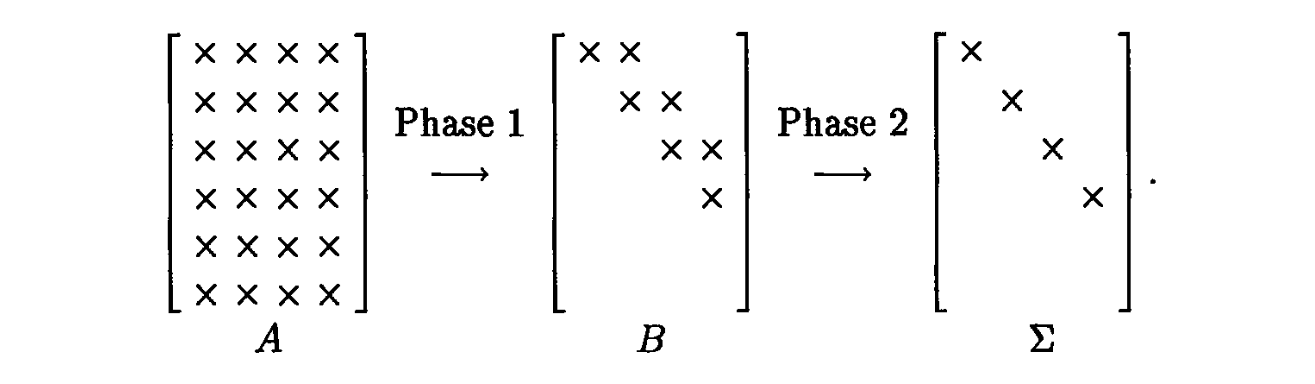
\includegraphics[width=0.8\textwidth]{figures/31-1.png}
 \end{figure}
 %────────────────────────────────────────
 Phase 1 involves $ O(mn^{2} ) $ flops. Phase 2 in principal requires an infinite number of operations, but the standard algorithms converge superlinearly, and thus only $ O(n\log(|\log(\mep)|)) $ iterations are needed for convergence to order $ \mep $. Because the matrix operated on is bidiagonal, each of these iterations requires only $ O(n) $ flops. Phase 2 therefore requires $ O(n^{2} ) $ flops all tother. Thus, although Phase 1 is finite and Phase 2 is in principle infinite, in practice the latter is much the less expensive, just as we found for the symmetric eigenvalue problem.  

 \section{Golub-Kahan Bidiagonalization} 
  Note that the difference to eigenvalue decomposition is that we don't similar transformation and we can completely triangularize and also introduce zeros above the first superdiagonal.  The simplest method for accomplishing this is the \textbf{Glub-Kahan bidiagonalization}.  House holder reflectors are applied alternately on the left and the right. For example 
  %────────────────────────────────────────
  \begin{figure}[H]
    \centering
    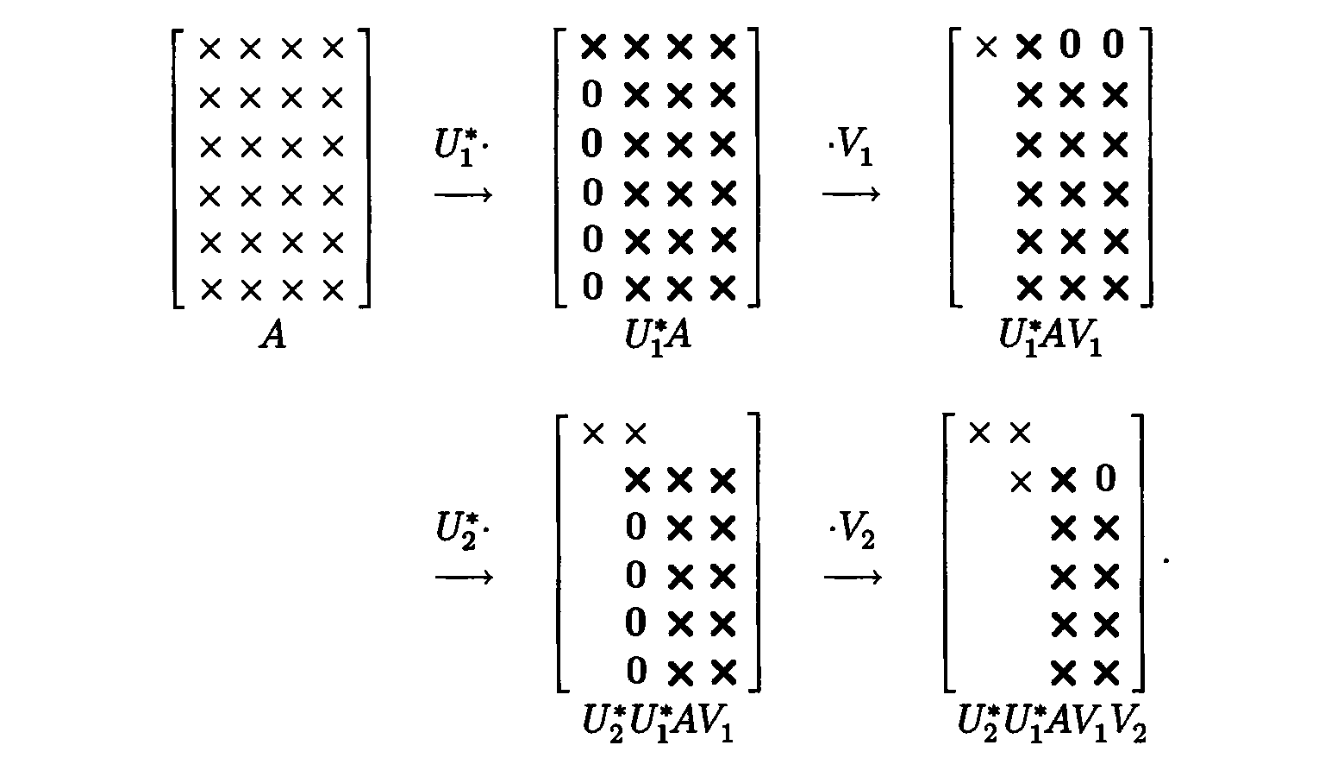
\includegraphics[width=0.8\textwidth]{figures/31-2.png}
  \end{figure}
  %────────────────────────────────────────
  At the end of this process, $n$ reflectors have been applied on the left and $n-2$ on the right. The total operation count is therefore twice that of a QR factorization. 


%────────────────────────────────────────
\begin{proposition}
\label{prop: Work for GK bi}
The work for Golub-Kahan bidiagonalization: $ \approx 4mn^{2}  - \frac{4}{3}n^3 $ flops. 
\end{proposition}
%────────────────────────────────────────

\section{Faster Methods for Phase 1} 
For $ m\gg n $, this operation count is unnecessarily large. A single QR factorization would introduce zeros everywhere below the diagonal, and for $ m\gg n $, there are the great majority of the zeros that are needed.  Hence, we can consider the an alternative method for bidiagonalization with with $ m\gg n $, first proposed by Lawson and Hanson and later developed by Chan. The idea, LHC bidiagonalization is illustrated as follows: 
%────────────────────────────────────────
\begin{figure}[H]
    \centering
    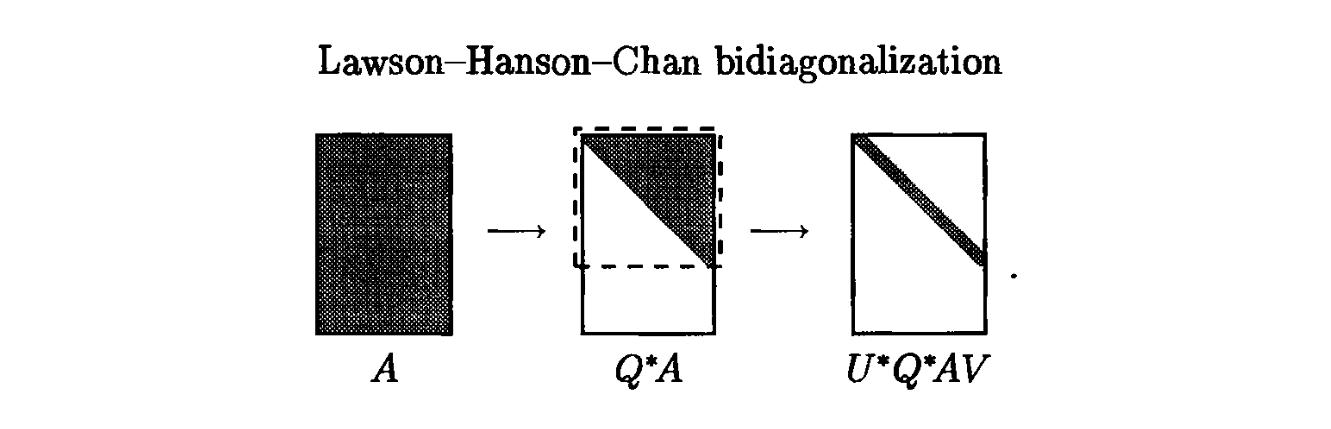
\includegraphics[width=0.9\textwidth]{figures/31-3.png}
\end{figure}
%────────────────────────────────────────
We do QR $A=QR$ first and then compute the Golub-Kahan bidiagonalization $B = U^*R V$ of $R$. The QR needs $ 2mn^{2}  - \frac{2}{3}n^3 $ flops (\autoref{cor: cost of QR}), and the Gould-Kahan procedure which requires $ \frac{8}{3}n^3 $ flops. The total operation count is: 


%────────────────────────────────────────
\begin{corollary}
\label{cor: cost of LHC}
The work for LHC bidiagonalization: $ \approx 2mn^{2}  + 2n^3 $ flops. 
\end{corollary}
%────────────────────────────────────────

This is cheaper than Golub-Kahan bidiagonalization for $ m>\frac{5}{3}n $. 

The LHC procure is advantageous only when $ m>\frac{5}{3}n $, but the idea can be generalized so as to realize a saving for any $ m>n $. The trick is to apply the QR not the beginning of the computation, but at a suitable point in the middle.  

%────────────────────────────────────────
\begin{figure}[H]
    \centering
    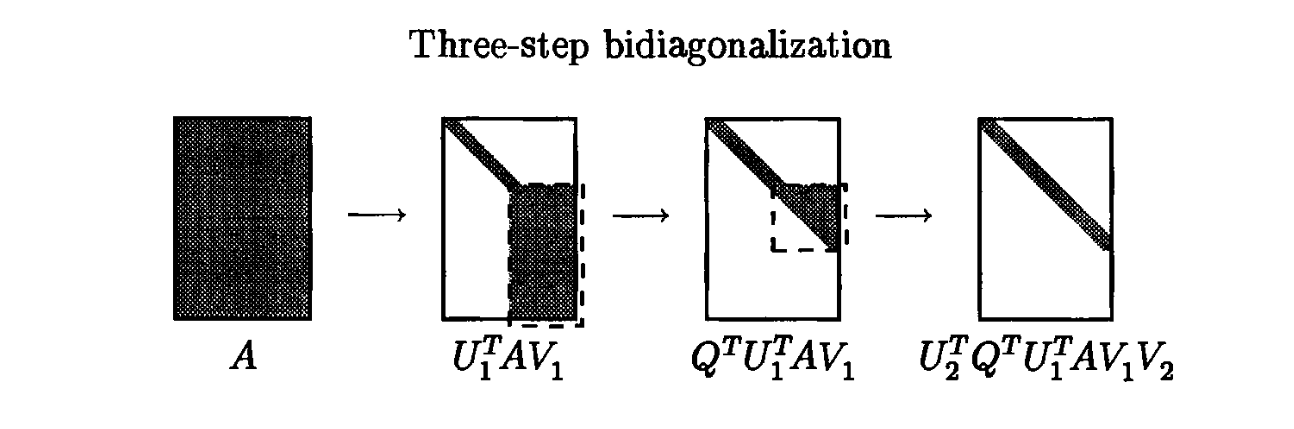
\includegraphics[width=0.9\textwidth]{figures/31-4.png}
\end{figure}
%────────────────────────────────────────

When should the QR factorization be performed? If we aim solely to minimize the operation count, the answer is simple: when the aspect ratio reaches $ (m-k)/(n-k) = 2 $. This choice leads to the formula: 


%────────────────────────────────────────
\begin{corollary}
\label{cor: cost of three-step bidiagonalization}
Work for three-step bidiagonalization: $ \sim 4mn^{2}  - \frac{4}{3}n^3 - \frac{2}{3}(m-n)^3 $ flops. 
\end{corollary}
%────────────────────────────────────────
This is a modest improvement over the other two methods for $n<m<2n$.  It must be admitted that the improvement achieved by the three-step method is small enough that in practice, other matters besides the count may determine which method is best on a real machine. 

%────────────────────────────────────────
\begin{figure}[H]
    \centering
    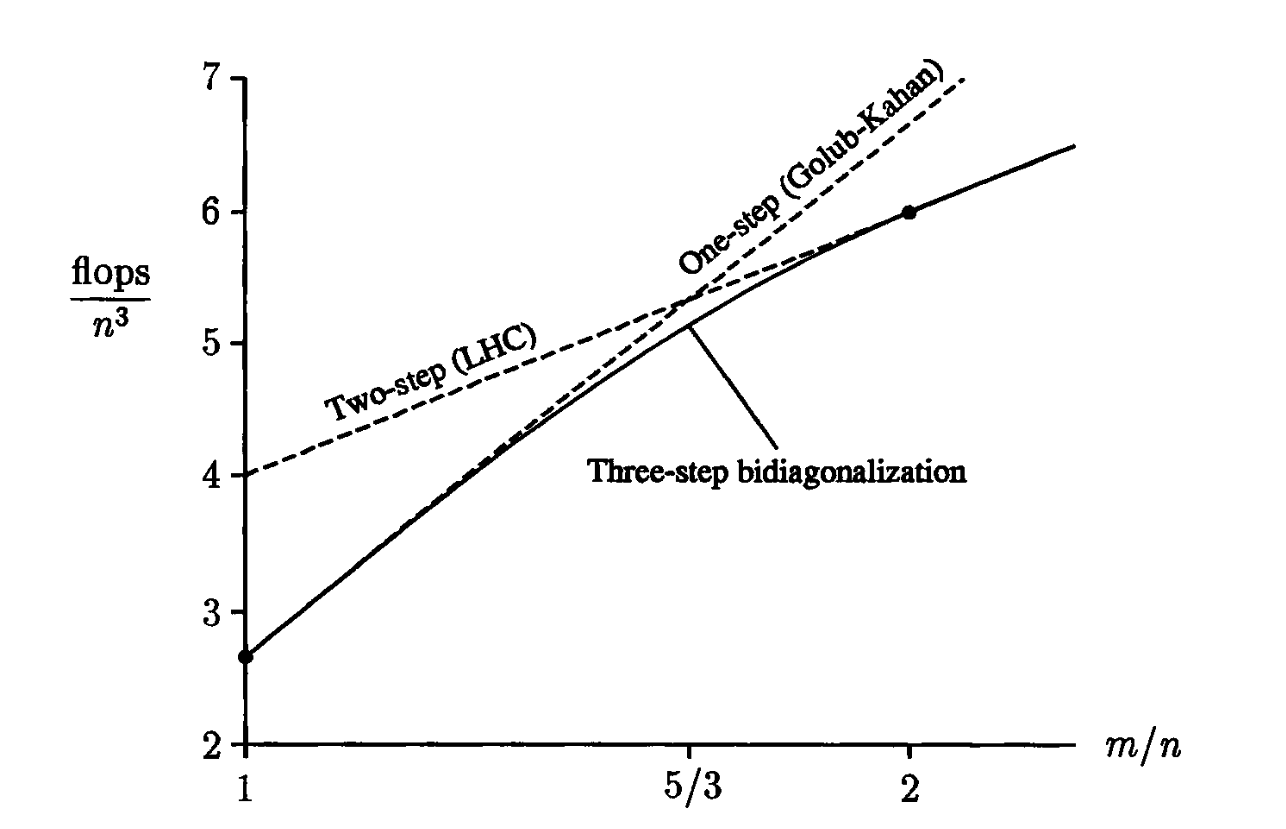
\includegraphics[width=0.8\textwidth]{figures/31-5.png}
    \caption{Operation counts for three bidiagonalization algorithms applied to $ m\times n $ matrices. Three-step bidiagonalization provides a pleasing smooth interpolant between the other two methods, thought the improvement is hardly large.}
\end{figure}
%────────────────────────────────────────

\section{Phase 2} 

In Phase 2 of the computation of the SVD, the SVD of the bidiagonal matrix B is determined. From the 1960s to the 1990s, the standard algorithm for this was a variant of the QR algorithm. More recently, divide-and-conquer algorithms have also become competitive, and in the future, they are likely to become the standard. We shall not give details.